%%%%%%%%%%%%%%%%%%%%%%%%%%%%%%%%%%%%%%%%%%%%%%%%%%%%%%%%%%%%%%%%%%%%%%%%
%    INSTITUTE OF PHYSICS PUBLISHING                                   %
%                                                                      %
%   `Preparing an article for publication in an Institute of Physics   %
%    Publishing journal using LaTeX'                                   %
%                                                                      %
%    LaTeX source code `ioplau2e.tex' used to generate `author         %
%    guidelines', the documentation explaining and demonstrating use   %
%    of the Institute of Physics Publishing LaTeX preprint files       %
%    `iopart.cls, iopart12.clo and iopart10.clo'.                      %
%                                                                      %
%    `ioplau2e.tex' itself uses LaTeX with `iopart.cls'                %
%                                                                      %
%%%%%%%%%%%%%%%%%%%%%%%%%%%%%%%%%%
%
%
% First we have a character check
%
% ! exclamation mark    " double quote  
% # hash                ` opening quote (grave)
% & ampersand           ' closing quote (acute)
% $ dollar              % percent       
% ( open parenthesis    ) close paren.  
% - hyphen              = equals sign
% | vertical bar        ~ tilde         
% @ at sign             _ underscore
% { open curly brace    } close curly   
% [ open square         ] close square bracket
% + plus sign           ; semi-colon    
% * asterisk            : colon
% < open angle bracket  > close angle   
% , comma               . full stop
% ? question mark       / forward slash 
% \ backslash           ^ circumflex
%
% ABCDEFGHIJKLMNOPQRSTUVWXYZ 
% abcdefghijklmnopqrstuvwxyz 
% 1234567890
%
%%%%%%%%%%%%%%%%%%%%%%%%%%%%%%%%%%%%%%%%%%%%%%%%%%%%%%%%%%%%%%%%%%%
%
\documentclass[10pt]{iopart}

\usepackage{citesort}

\usepackage{array}
\usepackage{textcomp}
\usepackage{graphicx}
\usepackage{stfloats}
\usepackage{float}
\usepackage{booktabs}
\usepackage{subcaption}
\usepackage{url}
%\usepackage{orcidlink}
%\usepackage{hyperref}
\usepackage{xcolor}
\usepackage{tikz}
\usetikzlibrary{arrows.meta, positioning, shapes.geometric}
\newcommand{\gguide}{{\it Preparing graphics for IOP Publishing journals}}

\newcommand{\BibTeX}{Bib\TeX}
\newcommand{\REVTeX}{REV\TeX}

\sloppy 
%Uncomment next line if AMS fonts required
%\usepackage{iopams}  



\bibliographystyle{iopart-num}

\begin{document}

\title[Validation of an EEG-based cognitive load index]
{Validation of a Theta/Alpha (Fz/Pz) EEG-Based Cognitive Load Index for Workload-Aware Human--Machine Systems}

\author{Edgar R. Hernandez-Rios$^1$$,^2$, 
Jerónimo Aparicio-Juarez$^1$, 
Christian Penaloza$^2$$,^3$,
Omar A. Dominguez-Ramirez$^1$}

\address{$^1$ Universidad Autonoma del Estado de Hidalgo (UAEH), Pachuca, Mexico}
\address{$^2$ Mirai Innovation Research Institute, Osaka, Japan}
\address{$^3$ Universidad Autonoma de Chihuahua (UACH), Chihuahua, Mexico}

\ead{omar@uaeh.edu.mx}

\begin{abstract}

Workload-aware intelligent human--machine systems require reliable and interpretable user-state estimation mechanisms. This study validates an EEG-based cognitive load index defined as the ratio of frontal theta to parietal alpha power ($\theta_{Fz}/\alpha_{Pz}$) across two complementary paradigms: a controlled laboratory benchmark and an ecological interactive task.

In the controlled paradigm, passive reading (low demand) and Stroop interference (high demand) were used to manipulate workload. Six sessions satisfying predefined signal-quality criteria consistently exhibited higher $\theta_{Fz}/\alpha_{Pz}$ ratios during high demand, with group means increasing from 1.37 (SD = 1.80) to 4.65 (SD = 4.99) and a paired Cohen's $d=0.75$, supporting discriminative validity under well-defined conditions. In the ecological paradigm, the index was baseline-normalized during interactive task execution; 6 of 8 sessions showed increased ratios relative to baseline, indicating sensitivity to task engagement under realistic interaction variability.

NASA-TLX scores were collected to contextualize perceived workload. Overall, the results support the $\theta_{Fz}/\alpha_{Pz}$ ratio as a compact, interpretable, and implementation-ready metric for cognitive load estimation, suitable for integration into workload-aware human--machine systems.

\end{abstract}

%
% Uncomment for keywords
\vspace{2pc}
\noindent{\it Keywords}: EEG, Cognitive load estimation, Theta/Alpha ratio, User-state estimation, Workload-aware systems, Human--machine interaction, Neuroergonomics, Exergaming.
%
% Uncomment for Submitted to journal title message
%\submitto{\JPA}
%
% Uncomment if a separate title page is required
%\maketitle
% 
% For two-column output uncomment the next line and choose [10pt] rather than [12pt] in the \documentclass declaration
%\ioptwocol
%

%\keywords{magnetic moment, solar neutrinos, astrophysics}
%\submitto{\jpg}

\ioptwocol

\maketitle


\section{Introduction}

Quantifying cognitive load from neurophysiological signals is a central challenge in neuroergonomics, adaptive human--machine interaction, and intelligent training systems. Reliable estimation of cognitive workload enables the characterization of how task demands influence attention, executive control, and performance, and constitutes a key component for the development of systems capable of adapting to the user’s cognitive state \cite{24}. In domains such as robotics, immersive virtual environments, and interactive training platforms, real-time awareness of user workload has the potential to improve safety, optimize task difficulty, and maintain effective interaction between humans and intelligent systems.

Maintaining cognitive workload within an optimal range is particularly important for human performance. According to the classical Yerkes--Dodson relationship, both insufficient cognitive engagement (underload) and excessive mental demand (overload) can negatively affect performance. Systems capable of monitoring user workload in real time therefore enable adaptive strategies such as dynamic task difficulty adjustment, intelligent assistance, or workload-aware feedback. In workload-aware human--machine systems, maintaining users within this optimal operating range is particularly relevant because both underload and overload may degrade performance, decision-making, and learning efficiency.

Among available sensing modalities, electroencephalography (EEG) has become one of the most widely used techniques for cognitive workload monitoring due to its high temporal resolution and its direct relationship with cortical processes underlying mental effort and attentional control. Numerous studies have demonstrated that specific spectral modulations in EEG activity are associated with variations in cognitive demand. In particular, increases in frontal theta activity (4--7~Hz) have been linked to executive control, conflict monitoring, and sustained attention, whereas decreases in parietal alpha activity (8--12~Hz) are commonly interpreted as markers of increased cortical engagement and information processing demand \cite{c8}. These spectral dynamics have been widely reported as robust EEG correlates of cognitive workload across experimental paradigms \cite{c1,c4}.

Frontal-midline theta activity has been specifically associated with cognitive control processes such as conflict monitoring and error processing, and is widely recognized as one of the most reliable spectral markers of mental effort \cite{CavanaghFrank2014_FrontalTheta}. In contrast, task-related alpha desynchronization—often prominent over posterior and parietal regions—reflects increased cortical engagement and active information processing due to a release of functional inhibition \cite{Klimesch2007_AlphaInhibitionTiming}. These complementary oscillatory dynamics provide a neurophysiological basis for constructing compact spectral indices capable of capturing variations in cognitive load.

Building on these findings, several studies have proposed ratio-based EEG metrics that combine theta and alpha activity into a single scalar indicator of cognitive load. Such ratios integrate complementary neural mechanisms—frontal executive engagement and parietal task-related desynchronization—while reducing feature dimensionality compared to multi-feature machine learning approaches. As a result, theta-to-alpha or alpha-to-theta ratios have been suggested as interpretable and computationally efficient workload indicators suitable for real-time monitoring in interactive systems \cite{c1,c7}. However, recent work emphasizes that the reliability and generalizability of EEG-based workload metrics depend strongly on methodological factors such as electrode configuration, preprocessing pipelines, artifact handling, and task context \cite{c4,c6,Mastropietro2023_ReliabilityFzPz}.

Despite the growing number of EEG-based workload metrics proposed in the literature, several methodological challenges remain. First, many studies rely on complex feature sets or machine learning models that are difficult to interpret and reproduce across laboratories. Second, validation is frequently performed only under tightly controlled experimental conditions, limiting the applicability of these approaches in real interactive environments. Third, differences in preprocessing pipelines, artifact rejection strategies, and electrode selection often make it difficult to compare results across studies. Standardized EEG preprocessing approaches have therefore been proposed to improve reproducibility and cross-study comparability \cite{BigdelyShamlo2015_PREP}. These challenges highlight the need for compact, interpretable workload indices validated through transparent processing pipelines and tested across both controlled and ecological task contexts.

Controlled cognitive interference paradigms, such as the Stroop task, are widely used as benchmarks for eliciting well-characterized increases in cognitive load. EEG studies consistently report increased frontal theta activity and modulation of alpha rhythms during Stroop interference, reflecting elevated executive and attentional demands \cite{c5,c9}. While these paradigms provide well-defined conditions for validating workload indices, many real-world human--machine systems operate in interactive environments where cognitive demand fluctuates dynamically and cannot be reduced to strictly scripted stimuli. Recent neuroergonomics studies demonstrate that EEG-based workload measures can also be observed in ecological tasks such as driving or real-flight monitoring, highlighting the importance of evaluating workload metrics under naturalistic interaction scenarios \cite{DiFlumeri2018_RealDrivingMWL,Dehais2019_RealFlightDryEEG}.

In this work, we investigate a compact EEG-based cognitive load index defined as the ratio of frontal theta power at Fz to parietal alpha power at Pz. This index combines two well-established spectral correlates of cognitive workload—frontal theta associated with executive control and parietal alpha desynchronization associated with increased cortical engagement—into a single interpretable metric. 
Figure~\ref{fig:study_overview} summarizes the conceptual framework of the study, illustrating how the controlled and ecological paradigms converge on a compact EEG-derived cognitive load index for validation across interaction contexts.

\begin{figure*}[t]\centering
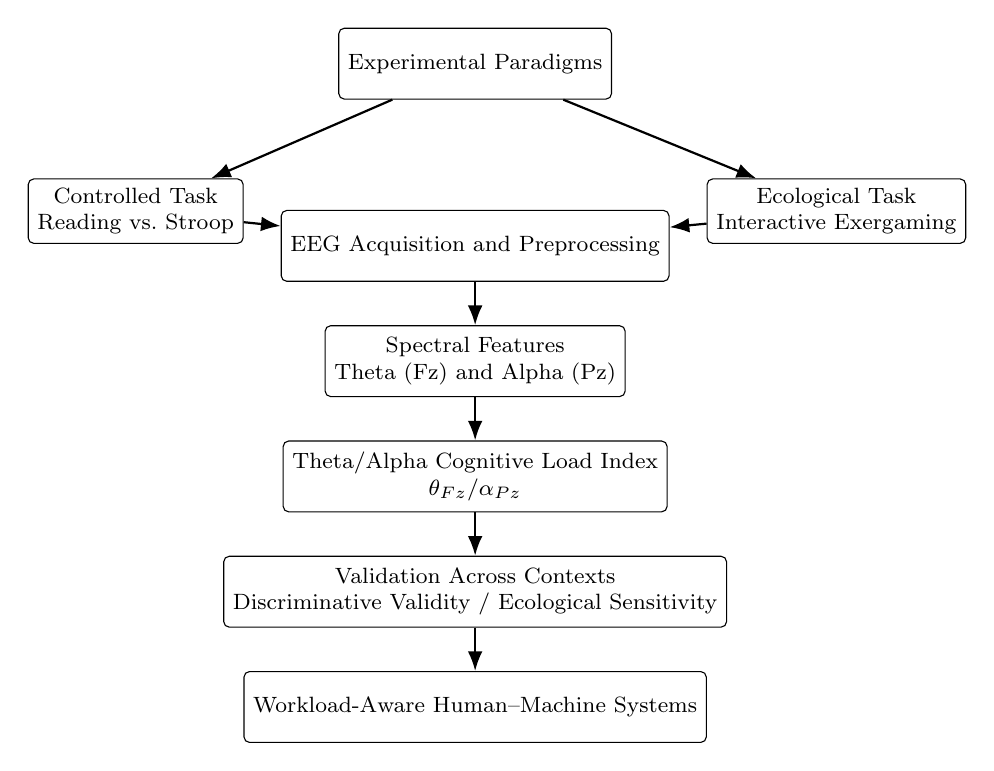
\begin{tikzpicture}[
    node distance=0.55cm and 0.9cm,
    every node/.style={font=\footnotesize, align=center},
    box/.style={
        draw,
        rounded corners=2pt,
        minimum width=2.9cm,
        minimum height=0.9cm,
        text centered
    },
    smallbox/.style={
        draw,
        rounded corners=2pt,
        minimum width=2.7cm,
        minimum height=0.8cm,
        text centered
    },
    arrow/.style={
        -{Latex[length=2.5mm]},
        thick
    }
]

\node[box] (paradigms) {Experimental Paradigms};

\node[smallbox, below left=1cm and 1.2cm of paradigms] (controlled)
{Controlled Task\\Reading vs.\ Stroop};

\node[smallbox, below right=1cm and 1.2cm of paradigms] (ecological)
{Ecological Task\\Interactive Exergaming};

\node[box, below=1.4cm of paradigms] (eeg) {EEG Acquisition and Preprocessing};

\node[box, below=of eeg] (features) {Spectral Features\\Theta (Fz) and Alpha (Pz)};

\node[box, below=of features] (index) {Theta/Alpha Cognitive Load Index\\$\theta_{Fz}/\alpha_{Pz}$};

\node[box, below=of index] (validation) {Validation Across Contexts\\Discriminative Validity / Ecological Sensitivity};

\node[box, below=of validation] (application) {Workload-Aware Human--Machine Systems};

\draw[arrow] (paradigms) -- (controlled);
\draw[arrow] (paradigms) -- (ecological);

\draw[arrow] (controlled) -- (eeg);
\draw[arrow] (ecological) -- (eeg);

\draw[arrow] (eeg) -- (features);
\draw[arrow] (features) -- (index);
\draw[arrow] (index) -- (validation);
\draw[arrow] (validation) -- (application);

\end{tikzpicture}
\caption{Conceptual overview of the study design. Two complementary paradigms—a controlled laboratory task and an ecological interactive task—are used to evaluate a compact EEG-based cognitive load index derived from frontal theta and parietal alpha activity.}
\label{fig:study_overview}
\end{figure*}

The main contributions of this work are threefold. First, we validate the $\theta_{Fz}/\alpha_{Pz}$ ratio under a controlled cognitive interference paradigm using predefined signal-quality criteria and session-level effect size analysis. Second, we examine the sensitivity of the same index in an ecological exergaming task involving sustained attention and sensorimotor coordination. Third, we present a transparent EEG processing pipeline that supports reproducibility and facilitates the integration of compact workload metrics into workload-aware human--machine systems.

%%%%%%%%%%%%%%%%%%%%%%%%%%%%%%%%%%%%%%%%%%%%%%%%%%%%%%%%%%%%%%%%%%%%%
\section{Experimental Context and Ecological Task Environment}

To evaluate the robustness of the proposed EEG-based cognitive load index across different interaction conditions, the study was designed around two complementary paradigms: a controlled cognitive workload benchmark and an ecological interactive task environment. The controlled paradigm provides well-defined experimental conditions that enable discriminative validation of the index, whereas the ecological paradigm introduces realistic variability associated with interactive human--machine systems. Together, these two contexts allow the assessment of both the internal validity and the ecological sensitivity of the proposed workload metric.

\subsection{Controlled experimental environment for cognitive load assessment}

A controlled experimental environment was developed to acquire and analyze electroencephalographic (EEG) signals during tasks designed to manipulate cognitive workload under well-defined conditions. The platform integrates standardized experimental tasks, a unified graphical interface for experiment control, real-time signal acquisition, and structured data recording. This configuration enables reproducible task timing, synchronized labeling of EEG data with experimental phases, and consistent data processing across participants and sessions.

The experimental protocol was designed to induce different levels of cognitive demand using tasks with well-established psychometric properties. The sequence included baseline conditions representing minimal cognitive demand, a low workload task involving passive processing, and a high workload task requiring attention and inhibitory control. This structure enables within-session comparison of EEG-derived workload indices across clearly differentiated cognitive load levels.

The protocol consisted of the following phases: a setup stage for signal verification and participant identification, a baseline period including 90~s with eyes open and 90~s with eyes closed, a low cognitive load condition of approximately 3~minutes consisting of passive text reading, and a high cognitive load condition of similar duration based on a cognitive interference task (Fig.~\ref{fig:controlled_protocol}).

\begin{figure}[t]
\centering
\resizebox{\columnwidth}{!}{%
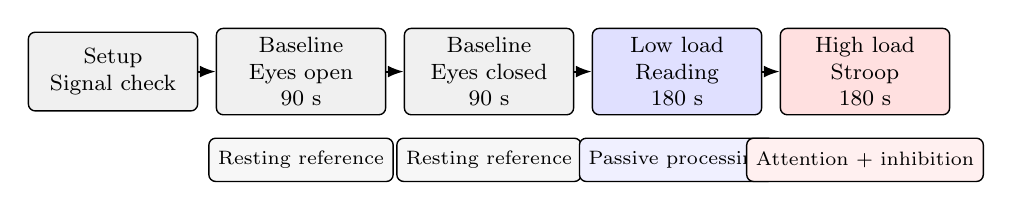
\begin{tikzpicture}[
    font=\footnotesize,
    node distance=0.22cm,
    phase/.style={
        draw,
        rounded corners=2.5pt,
        minimum width=2.15cm,
        minimum height=1.0cm,
        align=center,
        line width=0.5pt
    },
    phase_small/.style={
        draw,
        rounded corners=2.5pt,
        minimum width=2.15cm,
        minimum height=0.55cm,
        align=center,
        line width=0.5pt,
        font=\scriptsize
    },
    arrow/.style={
        -{Latex[length=2mm]},
        line width=0.7pt
    }
]

% Main row
\node[phase, fill=gray!12] (setup) {Setup\\Signal check};

\node[phase, fill=gray!12, right=of setup] (eo) {Baseline\\Eyes open\\90 s};

\node[phase, fill=gray!12, right=of eo] (ec) {Baseline\\Eyes closed\\90 s};

\node[phase, fill=blue!12, right=of ec] (low) {Low load\\Reading\\180 s};

\node[phase, fill=red!12, right=of low] (high) {High load\\Stroop\\180 s};

% Arrows
\draw[arrow] (setup) -- (eo);
\draw[arrow] (eo) -- (ec);
\draw[arrow] (ec) -- (low);
\draw[arrow] (low) -- (high);

% Bottom descriptors
\node[phase_small, fill=gray!6, below=0.28cm of eo] (ref1) {Resting reference};
\node[phase_small, fill=gray!6, below=0.28cm of ec] (ref2) {Resting reference};
\node[phase_small, fill=blue!6, below=0.28cm of low] (desc_low) {Passive processing};
\node[phase_small, fill=red!6, below=0.28cm of high] (desc_high) {Attention + inhibition};

\end{tikzpicture}%
}
\caption{Controlled experimental protocol used for cognitive load manipulation. After signal verification, participants completed resting baseline recordings, a low cognitive load condition based on passive reading, and a high cognitive load condition based on Stroop interference.}
\label{fig:controlled_protocol}
\end{figure}

The high-load condition was implemented using a Stroop color--word interference task, a classical paradigm widely used in cognitive neuroscience to elicit increased cognitive control demands. Participants were required to identify the ink color of visually presented words while suppressing the automatic tendency to read the written word. Stroop interference has been consistently associated with increased frontal theta activity and modulation of alpha-band dynamics in EEG recordings, reflecting heightened executive control and attentional demand \cite{c5,c9}. These well-characterized neurophysiological responses make the task an appropriate benchmark for validating EEG-based workload metrics.

The low-load condition consisted of passive reading of on-screen text without motor response requirements, providing a condition with minimal executive demand while maintaining visual engagement. Baseline recordings with eyes open and eyes closed served as reference conditions for signal quality verification and normalization procedures.

Experimental control and task presentation were implemented within a single graphical interface developed in Python using the PyQt framework. The interface integrates EEG device connectivity, real-time visualization of the recorded channels, task stimuli presentation, phase timers, and participant instructions. This unified environment ensures temporal synchronization between experimental phases and EEG acquisition, allowing each recorded sample to be associated with a labeled task condition for subsequent analysis.

Within the present study, this controlled environment provides the primary benchmark for evaluating whether the proposed Theta/Alpha (Fz/Pz) cognitive load index discriminates between clearly defined levels of cognitive demand.



\subsection{Ecological task environment: interactive exergaming platform}

While controlled laboratory tasks provide a reliable framework for validating EEG-based cognitive workload metrics, real-world human–machine interaction scenarios involve more complex and dynamic conditions. To evaluate the behavior of the proposed cognitive load index in a more ecologically valid context, the study incorporates an interactive exergaming environment developed in a complementary research project.

The exergaming platform integrates physical interaction, visual stimuli, and real-time system feedback, creating a task environment that more closely resembles natural human–technology interaction compared to traditional laboratory paradigms. Participants engage with the system through goal-directed movements while responding to visual elements presented within the game interface. This setup introduces simultaneous cognitive, perceptual, and motor demands that differ substantially from the isolated cognitive tasks used in controlled experimental protocols.

The platform combines a visual display presenting the interactive environment with motion-based user input, allowing participants to perform physical actions that directly influence the system behavior. The task requires continuous attention, perception of visual stimuli, and coordination of motor responses. These characteristics make exergaming environments increasingly relevant in research areas such as neuroergonomics, rehabilitation technologies, and adaptive human–machine systems.

The exergaming platform, referred to as \emph{K9 Canine Quest}, was developed as a multimodal interactive system integrating a virtual environment, multiple control modalities, and optional haptic feedback. Depending on the interaction mode, participants could engage with the task using keyboard, gamepad, or a haptic interface. In the haptic mode, the system provides force-feedback interaction through an articulated mechanism, allowing bidirectional coupling between user movement and the virtual task dynamics. This multimodal design enables the study of cognitive demand under interactive conditions that combine perception, action, and continuous task engagement.

During the interaction, EEG signals are continuously recorded using the same acquisition configuration employed in the controlled experimental protocol. This ensures methodological consistency when comparing neural indicators across experimental conditions. The ecological environment therefore provides an opportunity to examine whether the proposed cognitive workload index remains sensitive to variations in cognitive demand when users interact with a dynamic and physically engaging system.

Figure~\ref{fig:exergaming_platform} illustrates the exergaming setup used in the study, including the virtual environment, the haptic interface, and participant interaction during gameplay.

By incorporating this ecological interaction scenario, the study extends the evaluation of the EEG-based workload metric beyond controlled laboratory tasks, enabling preliminary assessment of its behavior under conditions that more closely resemble real-world human–machine interaction.

\begin{figure}[t]
\centering

\begin{subfigure}[t]{0.48\columnwidth}
\centering

\includegraphics[width=\linewidth]{figures/CQuest1.jpg}
\caption{Virtual environment used during the exergaming task.}
\end{subfigure}
\hfill
\begin{subfigure}[t]{0.48\columnwidth}
\centering
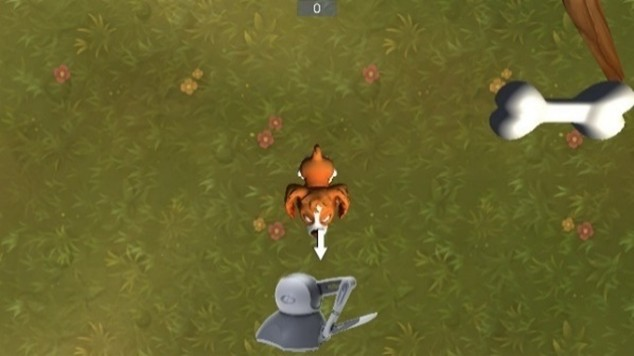
\includegraphics[width=\linewidth]{figures/CQuest2.jpg}
\caption{Haptic interface providing force-feedback interaction.}
\end{subfigure}

\vspace{0.4em}

\begin{subfigure}[t]{0.6\columnwidth}
\centering
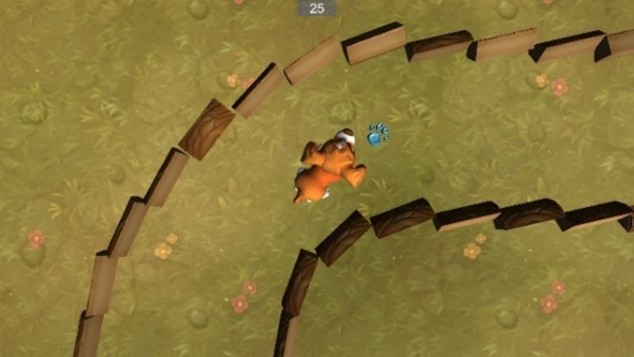
\includegraphics[width=\linewidth]{figures/CQuest4.jpg}
\caption{Participant interacting with the system during gameplay.}
\end{subfigure}

\caption{K9 Canine Quest exergaming platform used as an ecological interactive task environment. The system integrates virtual stimuli, haptic interaction, and user movement to create a physically and cognitively engaging task context while EEG signals are recorded.}

\label{fig:exergaming_platform}

\end{figure}

In the present work, the exergaming platform is not evaluated in terms of therapeutic efficacy or behavioral outcomes. Instead, it is used as an ecological interaction scenario for examining whether the proposed EEG-based cognitive load index remains sensitive under less constrained and more naturalistic task conditions.

\subsubsection{Exergaming platform architecture}

The ecological interaction task was implemented using the \textit{ADHD K9 CanineQuest} exergaming platform, a virtual environment designed to stimulate visuomotor coordination and attentional engagement during interactive tasks. The system integrates multiple interaction modalities with a controlled experimental logic to enable behavioral data collection alongside physiological measurements.

The operational logic of the platform is governed by a finite state machine (FSM) that coordinates the synchronization between visual stimuli, user interaction, and data acquisition processes. The FSM organizes the interaction into three main stages: baseline (rest), guided interaction, and active exploration. This structure allows consistent transitions between experimental phases while enabling the isolation of cognitive demands associated with different interaction conditions.

Three input modalities were implemented to explore variability in motor control and cognitive engagement: keyboard input, a standard gamepad controller, and a haptic articulated device. In the haptic modality, the system renders constant and spring-based force feedback, introducing additional sensorimotor coordination demands that may influence cognitive workload.

During the active exploration stage, participants maintain full control of spatial navigation within the virtual environment. From a motor control perspective, the interaction operates in an open-loop configuration in which the user's visuomotor responses determine the trajectory of movement within the virtual space.

The system records the kinematic state vector

\begin{equation}
\mathbf{P} = [x, y, z]^T
\end{equation}

and the interaction force vector

\begin{equation}
\mathbf{F} = [F_x, F_y, F_z]^T
\end{equation}

in real time during task execution.

Behavioral and interaction metrics are sampled at a temporal resolution of 0.01~s, generating a dataset that includes temporal interaction variables, spatial trajectory information, and force magnitudes. These behavioral measurements provide complementary information that contextualizes the EEG-derived cognitive workload index during ecological task execution.

The control structure underlying the active exploration mode is illustrated in Fig.~\ref{fig:ActiveHapticExploration_EN}.

\begin{figure*}[t]
   \centering
   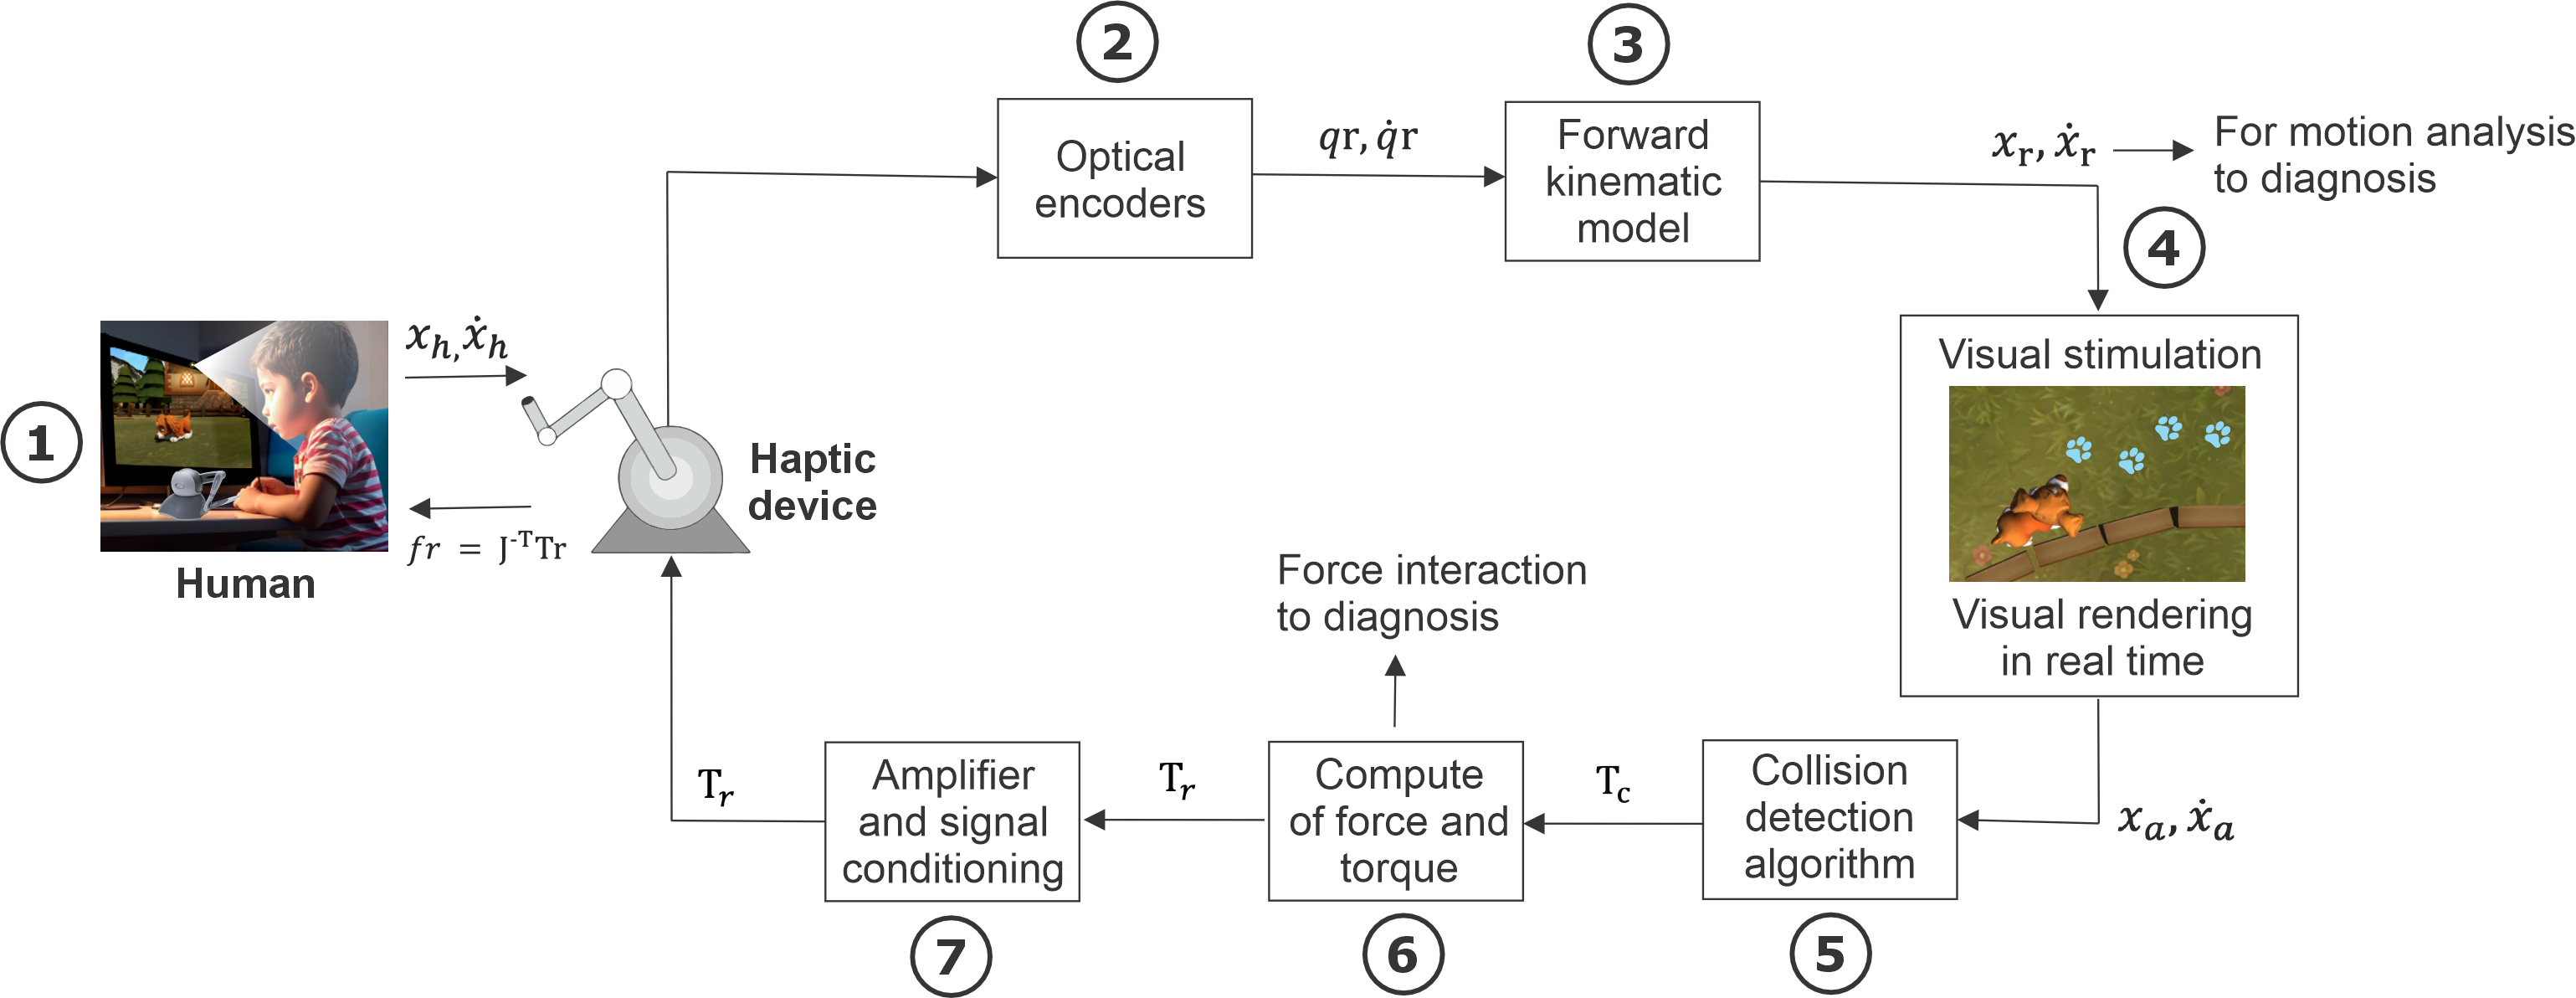
\includegraphics[width=\linewidth]{figures/ActiveHapticExploration_EN.png}
   \caption{Block diagram of the control loop implemented during the active exploration mode of the exergaming platform. The system captures user-generated motion commands and interaction forces while updating the virtual environment in real time, enabling the analysis of behavioral dynamics alongside physiological measurements.}
   \label{fig:ActiveHapticExploration_EN}
\end{figure*}

\subsection{Role of ecological interaction in workload validation}

A key challenge in EEG-based cognitive workload research is determining whether metrics validated under controlled laboratory conditions remain informative when applied to more realistic interactive settings. Controlled paradigms provide strong internal validity because task structure, duration, and cognitive demands can be defined with high precision. However, many human--machine systems operate in environments where user behavior is continuous, task demands fluctuate over time, and cognitive load emerges from the interaction between perception, action, and feedback rather than from isolated stimuli alone.

Within this context, the ecological exergaming paradigm complements the controlled benchmark by introducing sources of variability that are characteristic of real-world interaction, including multimodal input, sensorimotor coordination, movement-related noise, and individual differences in engagement strategy. These factors make ecological tasks less suitable for strict condition-by-condition comparisons, but particularly valuable for examining whether an EEG-derived workload index remains sensitive under more naturalistic conditions.

Accordingly, the two paradigms serve distinct but complementary validation purposes in this study. The controlled reading-versus-Stroop protocol is used to assess discriminative validity under well-defined cognitive load manipulation, whereas the ecological exergaming task is used to examine the sensitivity of the same index during continuous interactive behavior. This combined design allows evaluation of the proposed Theta/Alpha (Fz/Pz) ratio not only as a laboratory marker of workload differences, but also as a candidate metric for workload-aware human--machine systems operating outside tightly controlled settings.

Importantly, the ecological paradigm is not intended to provide the same level of experimental control as the laboratory benchmark, nor to support direct equivalence between paradigms. Rather, its role is to test whether the proposed index preserves interpretable task-related variation when cognitive demand arises in a dynamic interaction context. In this sense, the ecological component strengthens the practical relevance of the study by extending validation beyond strictly scripted tasks.
%%%%%%%%%%%%%%%%%%%%%%%%%%%%%%%%%%%%%%%%%%%%%%%%%%%%%%%%%%%%%%%%%%%%%%%%%%%%%
\section{Methods}

\subsection{Participants and data overview}

EEG recordings were collected across two experimental paradigms: a controlled cognitive workload protocol and an ecological interactive exergaming task. The controlled protocol included a baseline phase followed by low and high cognitive workload conditions, whereas the ecological paradigm consisted of interactive task execution within the exergaming environment described in Section~II.

In total, 14 recording sessions were obtained for the controlled paradigm and 8 sessions for the ecological paradigm. Because EEG recordings collected during interactive tasks are susceptible to artifacts arising from eye movements, muscle activity, and motion-related noise, predefined signal-quality criteria were applied prior to analysis. These criteria ensured that spectral estimates used to compute the cognitive load index were derived from sufficiently clean signal segments.

Sessions that satisfied the predefined artifact thresholds and retained a minimum number of valid analysis windows were included in the primary controlled analysis. After applying these criteria, six sessions remained suitable for controlled Low–High workload comparison. Ecological sessions were analyzed using session-level baseline normalization to evaluate sensitivity of the workload index under interactive task conditions.   

\subsection{EEG acquisition}

EEG signals were recorded using the AURA biosensing system (Mirai Innovation Research Institute, Japan), an 8-channel EEG device with a nominal sampling rate of 250~Hz. Signals were streamed in real time using the Lab Streaming Layer (LSL) framework.

Electrodes were positioned according to the international 10--20 system at Fp1, Fp2, F3, Fz, F4, P3, Pz, and P4, covering bilateral frontopolar, frontal, and parietal regions as well as the midline. The cognitive load index investigated in this work was computed using theta-band activity from the frontal midline electrode (Fz) and alpha-band activity from the parietal electrode (Pz). This selection was motivated by prior literature linking frontal theta increases and parietal alpha suppression to elevated cognitive workload.

A custom graphical interface implemented in PyQt5 was used to guide the experimental protocol, present task stimuli, and store recorded EEG data as CSV files for offline processing.

\subsection{Signal preprocessing}

All EEG recordings were processed offline using a standardized preprocessing pipeline. Signals were first notch filtered at 60~Hz (quality factor $Q = 30$) to attenuate power-line interference. A fourth-order Butterworth bandpass filter between 1 and 40~Hz was subsequently applied to isolate the frequency range of interest for cognitive workload analysis.

Common average reference (CAR) was applied in the ecological paradigm to improve robustness against movement-related noise inherent to interactive tasks. In contrast, the controlled paradigm was analyzed using the original acquisition reference configuration to preserve comparability with the recording setup and minimize additional signal transformations.

The effective sampling rate was assumed to be 250~Hz and verified when necessary using signal timestamps recorded in the data streams.

\begin{figure}[t]
\centering
\resizebox{0.42\columnwidth}{!}{%
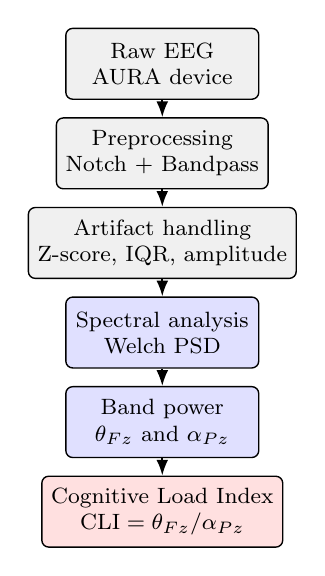
\begin{tikzpicture}[
    font=\footnotesize,
    node distance=0.22cm,
    phase/.style={
        draw,
        rounded corners=2.5pt,
        minimum width=2.45cm,
        minimum height=0.9cm,
        align=center,
        line width=0.5pt
    },
    arrow/.style={
        -{Latex[length=2mm]},
        line width=0.7pt
    }
]

\node[phase, fill=gray!12] (raw) {Raw EEG\\AURA device};

\node[phase, fill=gray!12, below=of raw] (pre) {Preprocessing\\Notch + Bandpass};

\node[phase, fill=gray!12, below=of pre] (artifact) {Artifact handling\\Z-score, IQR, amplitude};

\node[phase, fill=blue!12, below=of artifact] (psd) {Spectral analysis\\Welch PSD};

\node[phase, fill=blue!12, below=of psd] (bands) {Band power\\$\theta_{Fz}$ and $\alpha_{Pz}$};

\node[phase, fill=red!12, below=of bands] (cli) {Cognitive Load Index\\$\mathrm{CLI}=\theta_{Fz}/\alpha_{Pz}$};

\draw[arrow] (raw) -- (pre);
\draw[arrow] (pre) -- (artifact);
\draw[arrow] (artifact) -- (psd);
\draw[arrow] (psd) -- (bands);
\draw[arrow] (bands) -- (cli);

\end{tikzpicture}%
}
\caption{EEG processing pipeline used to compute the Cognitive Load Index (CLI). Raw EEG signals were preprocessed, artifact-contaminated segments were handled, spectral power was estimated using Welch’s PSD, and the CLI was computed as the ratio between frontal theta power (Fz) and parietal alpha power (Pz).}
\label{fig:eeg_pipeline}
\end{figure}

\subsection{Spectral analysis and Cognitive Load Index}

Spectral power was estimated using Welch’s power spectral density (PSD) method. EEG signals were segmented into windows of 250 samples (1~s at 250~Hz) with 50\% overlap (step size of 125 samples).

For each window, theta-band power (4--7~Hz) was computed from channel Fz and alpha-band power (8--12~Hz) from channel Pz. Bandpower was defined as the integral of the PSD over the corresponding frequency band using the trapezoidal rule.

The Cognitive Load Index (CLI) was defined for each window as:

\begin{equation}
\mathrm{CLI} = \frac{\theta_{Fz}}{\alpha_{Pz}}.
\label{CLI2}
\end{equation}

Non-finite values were discarded and division by zero was avoided. Index values were averaged across valid windows within each phase or session.

An overview of the EEG processing pipeline and index computation is shown in Fig.~\ref{fig:eeg_pipeline}.

\subsection{Artifact detection and window selection}

Artifacts were detected independently for channels Fz and Pz using three criteria: a Z-score threshold of 3, an interquartile range (IQR) threshold with a multiplier of 3, and an absolute amplitude threshold of 200~$\mu$V.

Artifact-contaminated samples were handled using linear interpolation when sufficient surrounding data were available in order to preserve temporal continuity. Segments with excessive contamination were excluded from analysis.

After artifact handling, the cognitive load index was recomputed. Only windows with finite index values within a predefined range (0.01--100) were retained. A minimum of two valid windows per phase was required to compute session-level averages, ensuring that estimates reflected more than isolated spectral events.

In some sessions, strict artifact rejection resulted in a limited number of valid analysis windows. This reflects the conservative nature of the predefined signal-quality criteria, particularly under conditions of frontal or parietal contamination. Because the objective of this study was to evaluate session-level trends and discriminative directionality of the index rather than window-level inference, sessions with at least two valid windows were retained to avoid discarding usable recordings while preserving methodological transparency.
To clarify the relationship between the two task contexts analyzed in this study, the experimental paradigms are summarized in Fig.~\ref{fig:protocol}.
\begin{figure}[t]
\centering
\resizebox{\columnwidth}{!}{%
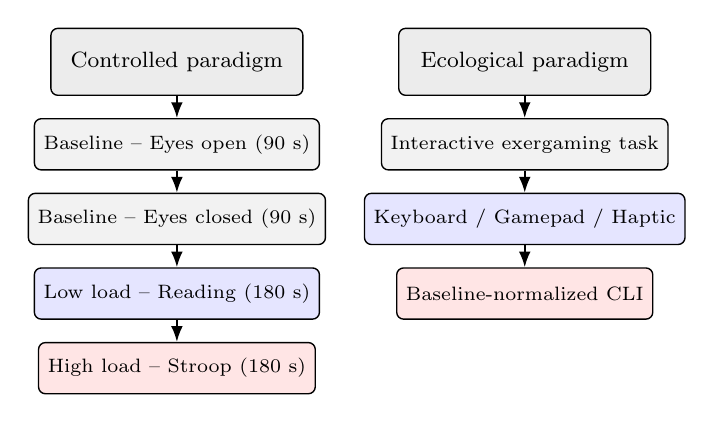
\begin{tikzpicture}[
    font=\footnotesize,
    node distance=0.28cm,
    phase/.style={
        draw,
        rounded corners=2.5pt,
        minimum width=3.2cm,
        minimum height=0.85cm,
        align=center,
        line width=0.5pt
    },
    smallphase/.style={
        draw,
        rounded corners=2.5pt,
        minimum width=2.9cm,
        minimum height=0.65cm,
        align=center,
        line width=0.5pt,
        font=\scriptsize
    },
    arrow/.style={
        -{Latex[length=2mm]},
        line width=0.7pt
    }
]

% Controlled paradigm
\node[phase, fill=gray!15] (ctrl) {Controlled paradigm};

\node[smallphase, fill=gray!10, below=of ctrl] (b1) {Baseline -- Eyes open (90 s)};
\node[smallphase, fill=gray!10, below=of b1] (b2) {Baseline -- Eyes closed (90 s)};
\node[smallphase, fill=blue!10, below=of b2] (low) {Low load -- Reading (180 s)};
\node[smallphase, fill=red!10, below=of low] (high) {High load -- Stroop (180 s)};

\draw[arrow] (ctrl) -- (b1);
\draw[arrow] (b1) -- (b2);
\draw[arrow] (b2) -- (low);
\draw[arrow] (low) -- (high);

% Ecological paradigm
\node[phase, fill=gray!15, right=1.2cm of ctrl] (eco) {Ecological paradigm};

\node[smallphase, fill=gray!10, below=of eco] (task) {Interactive exergaming task};
\node[smallphase, fill=blue!10, below=of task] (mod) {Keyboard / Gamepad / Haptic};
\node[smallphase, fill=red!10, below=of mod] (norm) {Baseline-normalized CLI};

\draw[arrow] (eco) -- (task);
\draw[arrow] (task) -- (mod);
\draw[arrow] (mod) -- (norm);

\end{tikzpicture}%
}
\caption{Overview of the experimental paradigms used in this study. The controlled protocol consisted of baseline recordings followed by low and high cognitive workload conditions. The ecological paradigm consisted of an interactive exergaming task performed with multiple interaction modalities and analyzed using baseline-normalized workload estimates.}
\label{fig:protocol}
\end{figure}
\subsection{Experimental paradigms}
\subsubsection{Controlled cognitive load protocol}

The controlled paradigm followed a baseline--low--high workload protocol.

After an initial signal verification phase, participants completed a baseline consisting of 90~s with eyes open followed by 90~s with eyes closed.

The low cognitive load condition consisted of passive reading for approximately 3 minutes. The high cognitive load condition consisted of a Stroop color--word interference task of comparable duration, in which participants identified the ink color rather than the written word using keyboard inputs (R/B/G/Y).

A session was considered \emph{includable} if, in both low and high load phases, the artifact percentage in either Fz or Pz did not exceed 50\% and at least two valid analysis windows remained after preprocessing.

Among includable sessions, the primary hypothesis tested was that the mean cognitive load index would be higher in the high-demand condition than in the low-demand condition (High $>$ Low).

\subsubsection{Ecological exergaming paradigm}

The ecological paradigm involved an interactive exergaming scenario implemented on the platform described in Section~II. The system supported keyboard, gamepad, and haptic interaction modalities.

Because ecological recordings did not contain explicit low/high phase labels, task segments were identified using event markers and segmented into pre-task baseline and active task periods.

Baseline values were obtained from within-session baselines when available; otherwise, baseline recordings from the controlled paradigm for the same participant were used to reduce inter-individual variability.

A normalized workload index was computed as

\begin{equation}
\mathrm{CLI}_{\mathrm{norm}} =
\frac{\mathrm{CLI}_{\mathrm{task}}}{\mathrm{CLI}_{\mathrm{baseline}}}
\label{eq:cli_norm}
\end{equation}

where values greater than 1 indicate increased workload during task execution relative to baseline.

\subsection{Subjective cognitive workload assessment}

Subjective cognitive workload was assessed using the NASA Task Load Index (NASA-TLX), a multidimensional questionnaire capturing Mental Demand, Physical Demand, Temporal Demand, Performance, Effort, and Frustration.

Raw (unweighted) NASA-TLX scores were computed and reported as percentages (0--100).

For the controlled paradigm, NASA-TLX was collected as a single global score per participant reflecting the overall session and was therefore not used for within-session Low vs.\ High comparisons.

For the ecological paradigm, NASA-TLX scores were collected after task completion for each interaction modality when available and were used descriptively to contextualize perceived workload.

\subsection{Statistical analysis}

For the controlled paradigm, index values were averaged per session within the low and high cognitive load phases. Group-level descriptive statistics (mean and standard deviation) were computed across includable sessions.

Effect size was quantified using paired Cohen’s $d$ computed on session-wise differences (High minus Low).

Given the modest number of includable controlled sessions and conservative artifact rejection, the analysis emphasizes descriptive statistics, directionality of the workload index, and paired effect size rather than inferential $p$-values.

\subsection{Dataset limitations and signal quality considerations}

The present study prioritized conservative signal-quality criteria in order to ensure reliable estimation of spectral features used for the cognitive load index. As a result, several recorded sessions were excluded from the controlled paradigm analysis due to excessive artifact contamination in frontal or parietal channels.

Specifically, recordings were considered includable only when the percentage of artifact-contaminated samples did not exceed 50\% in either Fz or Pz and when at least two valid analysis windows remained after preprocessing. These criteria reduced the number of usable sessions in the controlled dataset but ensured that reported index values were computed from segments with acceptable signal quality.

This conservative approach reflects the practical challenges of acquiring EEG in interactive and semi-naturalistic environments, where motion artifacts, electrode displacement, and environmental noise can affect signal integrity. Rather than relaxing artifact thresholds, the analysis preserved strict preprocessing criteria to maintain methodological transparency and reliability of the extracted workload index.

Because the objective of the study is to evaluate the directional behavior and feasibility of the proposed workload index across controlled and ecological conditions, analyses focus on session-level trends and effect sizes rather than large-sample statistical inference.
%%%%%%%%%%%%%%%%%%%%%%%%%%%%%%%%%%%%%%%%%%%%%%%%%%%%%%%%%%%%%%%%%%%%%
\section{Results}
This section reports the results obtained from both the controlled cognitive workload protocol and the ecological exergaming paradigm. Results are presented at the session level to reflect the preprocessing criteria and signal-quality constraints described in the Methods section.

\subsection{Controlled paradigm: low vs.\ high cognitive load}

From a total of 14 recorded sessions, six satisfied the predefined signal-quality inclusion criteria (artifact percentage in Fz or Pz $\leq$ 50\% and at least two valid windows after cleaning in both Low and High phases). These includable sessions were used for the primary controlled analysis. At the session level, all included sessions exhibited higher mean Theta/Alpha ratios in the high-demand condition (Stroop interference) than in the low-demand condition (passive reading), consistent with the expected direction of the workload hypothesis (High > Low).

Table~\ref{tab:controlled} reports per-session mean Theta/Alpha (Fz/Pz) ratios for Low and High conditions, the number of valid analysis windows retained after artifact handling, and the maximum artifact percentage across Fz and Pz in each condition. Despite marked inter-session variability in absolute ratio values and the limited number of valid windows in some sessions, the direction of change (High $>$ Low) was consistent across all included sessions.

\begin{table*}[tbp]
\centering
\caption{\raggedright Per-session summary for the controlled paradigm: mean Theta/Alpha (Fz/Pz) ratio in Low and High Load, valid windows after cleaning, and maximum artifact percentage (Fz or Pz) in each condition.}
\label{tab:controlled}
\footnotesize
\setlength{\tabcolsep}{8pt}
\begin{tabular}{c c c c c}
\toprule
\textbf{Session} & \textbf{Mean Low} & \textbf{Mean High} & \textbf{Valid win (L/H)} & \textbf{Max art.\ \% (L/H)} \\
\midrule
S1 & 3.94 & 6.69  & 2 / 2   & 2.57 / 2.14 \\
S2 & 0.09 & 0.10  & 2 / 2   & 2.36 / 1.06 \\
S3 & 0.30 & 11.36 & 2 / 2   & 2.96 / 26.51 \\
S4 & 0.10 & 0.43  & 59 / 64 & 16.46 / 10.07 \\
S5 & 0.35 & 0.39  & 2 / 2   & 1.92 / 29.15 \\
S6 & 3.42 & 8.97  & 2 / 2   & 7.04 / 4.03 \\
\bottomrule
\end{tabular}
\end{table*}

Sessions with a limited number of valid windows are reported explicitly to ensure transparency and should be interpreted as conservative estimates of session-level index behavior.

At the group level, the mean Theta/Alpha ratio increased from 1.37 (SD = 1.80) during Low Load to 4.65 (SD = 4.99) during High Load, yielding a mean difference (High $-$ Low) of 3.29. The corresponding paired Cohen’s $d$, computed on session-wise differences, was 0.75, indicating a medium effect size. Fig.~\ref{fig:paired_slope} illustrates the Low vs.\ High comparison for each included session.

\begin{figure}[t]
\centering
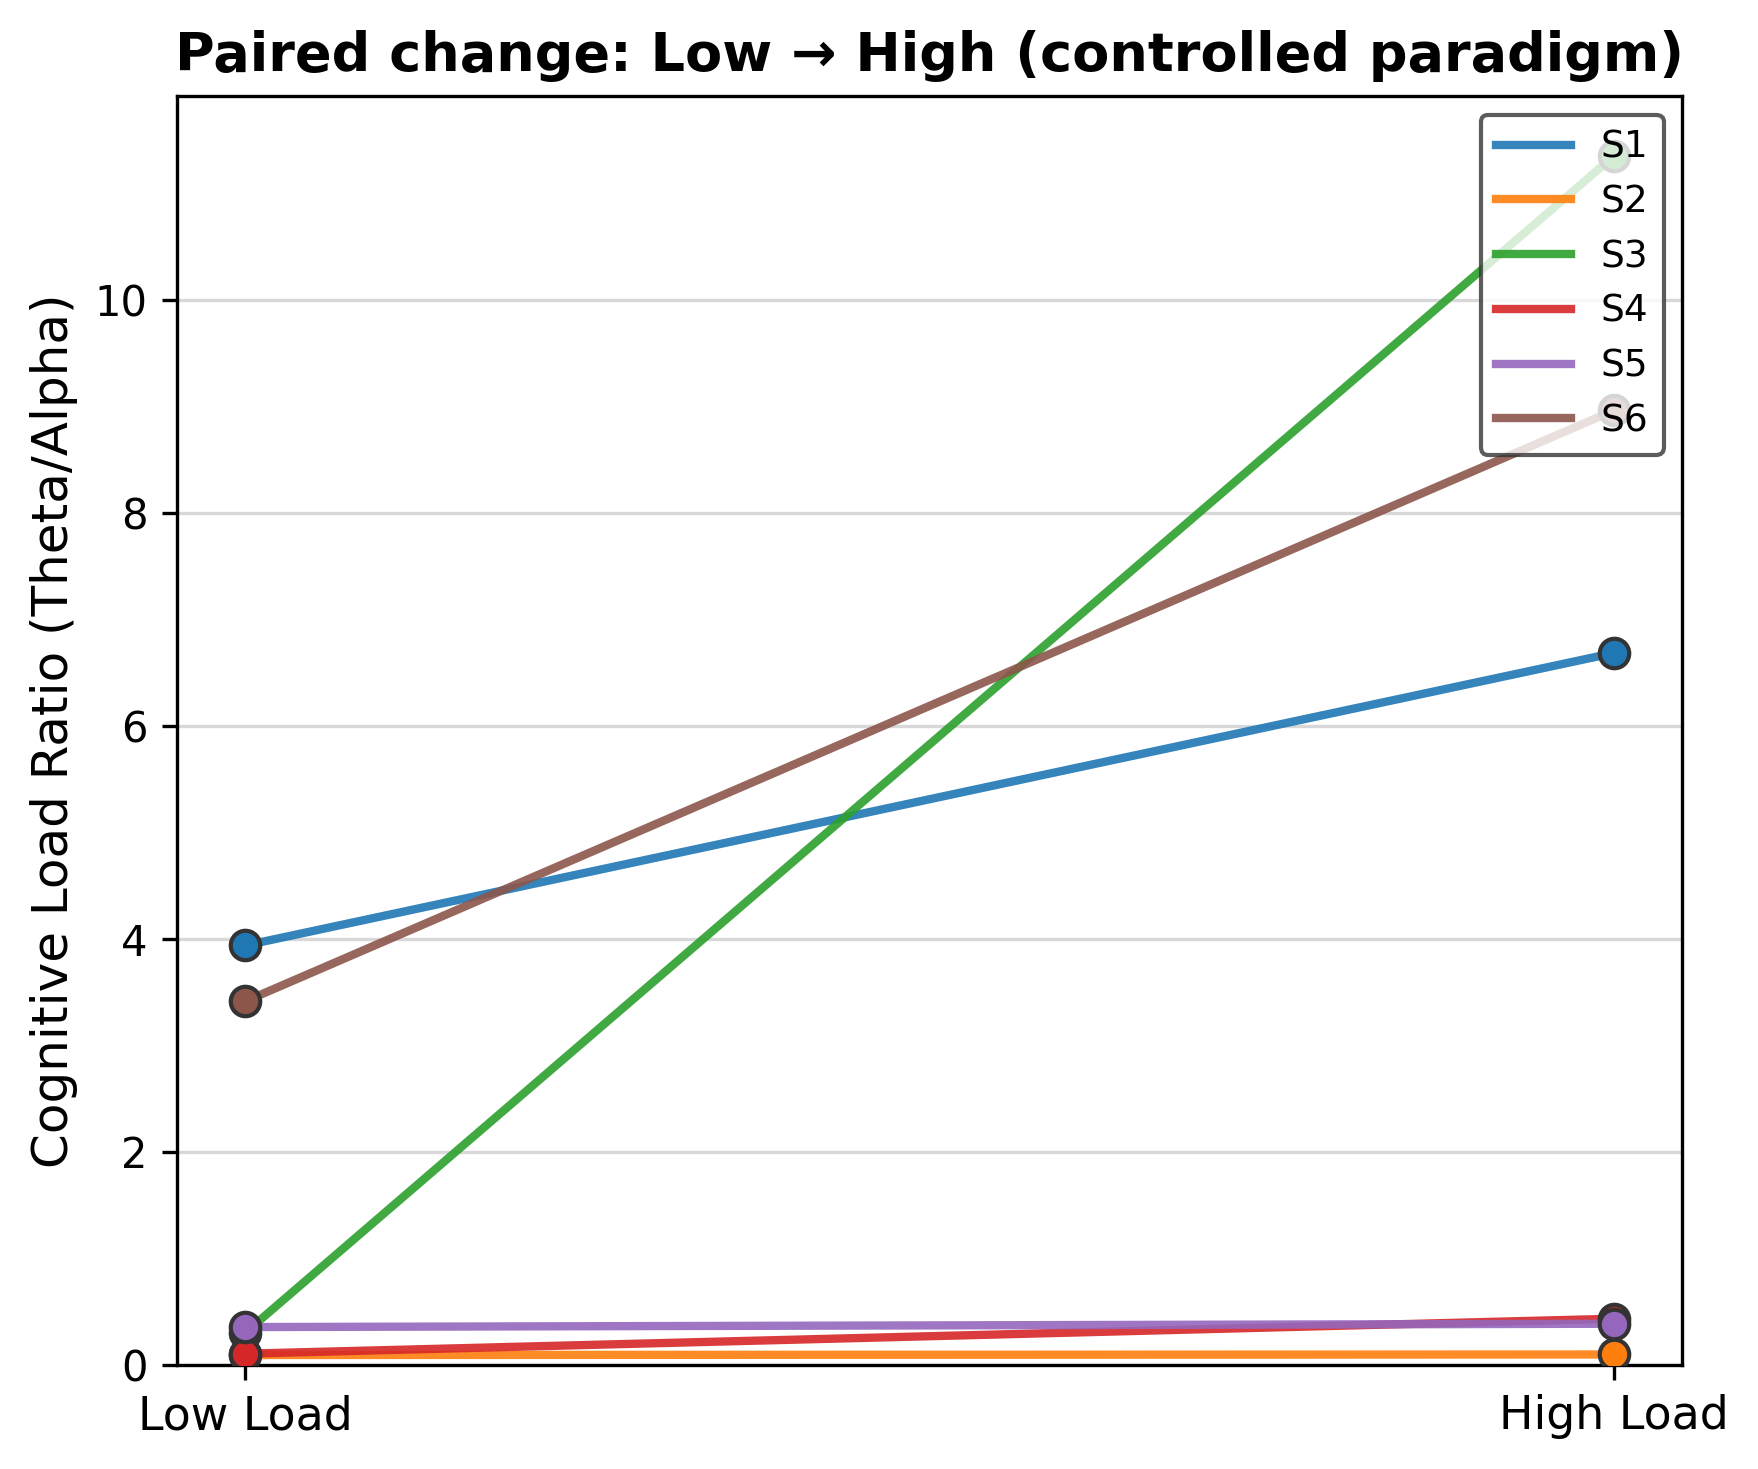
\includegraphics[width=0.7\linewidth]{figures/cumplen_incluibles_paired_slope.png}
\caption{Paired slope plot: Theta/Alpha (Fz/Pz) ratio for each of the six includable sessions from Low Load to High Load (controlled paradigm). Each line represents one session; all lines show an increase, consistent with the hypothesis.}
\label{fig:paired_slope}
\end{figure}

\subsection{Ecological paradigm: exergaming task (baseline-normalized)}

For the ecological exergaming paradigm, analysis was conducted at the session level using recordings that contained an identifiable task segment suitable for baseline comparison. The Theta/Alpha ratio was computed using the same index definition (Fz/Pz) and normalized relative to each session’s baseline value (Equation \ref{CLI}).

%\[
%\mathrm{Index}_{\mathrm{norm}} = \frac{\mathrm{Index}_{\mathrm{task}}}{\mathrm{Index}_{\mathrm{baseline}}}.
%\]
Normalized values greater than 1 indicate higher index values during the task segment relative to baseline.

Across eight analyzed sessions, six exhibited $\mathrm{Index}_{\mathrm{norm}} > 1$ (task $>$ baseline), while two sessions showed $\mathrm{Index}_{\mathrm{norm}} < 1$ (task $<$ baseline). Sessions with $\mathrm{Index}_{\mathrm{norm}} > 1$ yielded normalized ratios of 7.85, 1.87, 2.51, 3.14, 4.08, and 2.14, whereas the remaining two sessions yielded normalized ratios of 0.71 and 0.33.

Figure~\ref{fig:eco_norm} summarizes the baseline-normalized Theta/Alpha (Fz/Pz) ratio for each ecological session. Session identifiers (S1--S8) correspond to recording sessions and do not necessarily represent unique participants, as some participants completed multiple sessions using different interaction modalities. Values above unity indicate increased cognitive load during task execution relative to baseline, whereas values below unity are reported without overinterpretation and may reflect individual differences, baseline selection, or variability in task engagement.

\begin{figure}[t]
    \centering
    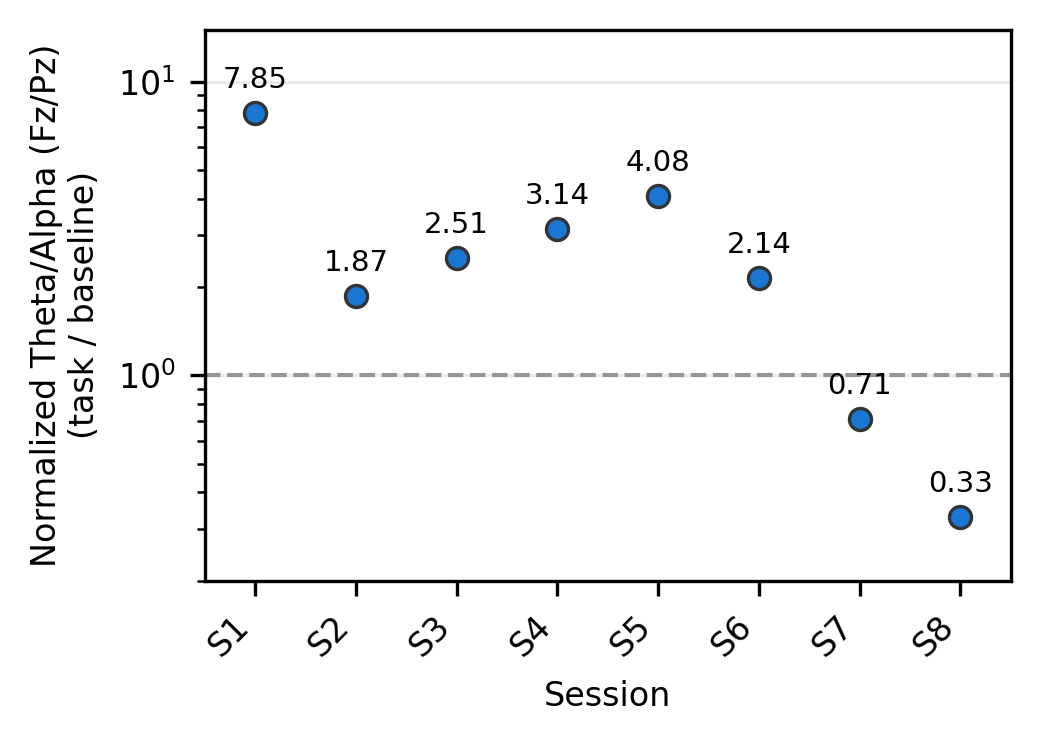
\includegraphics[width=\linewidth]{figures/eco_normalized_ratio_log.png}
    \caption{Ecological paradigm: baseline-normalized Theta/Alpha (Fz/Pz) ratio during the task segment (task/baseline). The dashed line indicates the unity reference (no change relative to baseline).}
    \label{fig:eco_norm}
\end{figure}

\subsection{Subjective workload results}

NASA-TLX scores were used to provide complementary subjective estimates of perceived workload. For the controlled paradigm, a single global NASA-TLX score was collected per participant for the overall session, yielding a mean workload of 48.8\% (SD = 13.5, $N=10$). Because NASA-TLX was not administered separately for Low and High phases, no within-session subjective comparison was performed.

For the ecological exergaming paradigm, NASA-TLX scores were collected per interaction modality when available. Mean subjective workload values were 41.4\% (SD = 14.1) for the Haptic modality, 35.3\% (SD = 13.8) for the Gamepad modality, and 44.1\% (SD = 15.2) for the Keyboard modality ($N=10$). Among the three modalities, the Gamepad condition exhibited the lowest perceived workload on average.

Overall, NASA-TLX results indicate moderate subjective workload across both paradigms and provide contextual information that complements the EEG-derived cognitive load indices without implying direct correspondence at the session or phase level.

%%%%%%%%%%%%%%%%%%%%%%%%%%%%%%%%%%%%%%%%%%%%%%%%%%%%%%%%%%%%%%%%%%%%%%%%%%%%%%%%%%%%%%%%%%%%%%%%%%%%%%
\section{Discussion}

The results obtained in the controlled paradigm support the expected behavior of the proposed Theta/Alpha (Fz/Pz) cognitive load index. Across all includable sessions, the index increased from the passive reading condition to the Stroop interference task, which represents a higher cognitive demand scenario. This directional consistency aligns with established neurophysiological findings linking increases in frontal theta activity and reductions in parietal alpha activity with elevated cognitive workload and executive control demands \cite{c1,c4,c5,c9}. Although the number of includable sessions was limited due to conservative signal-quality criteria, the observed session-level trends and the medium effect size obtained at the group level suggest that the index captures meaningful variations in cognitive demand under controlled experimental conditions.

The ecological exergaming paradigm provides a complementary perspective on the behavior of the index under more naturalistic interaction conditions. In the majority of analyzed sessions, the baseline-normalized Theta/Alpha ratio increased during task execution relative to baseline, suggesting sensitivity to the cognitive and sensorimotor demands introduced by the interactive environment. Compared to the controlled benchmark, the ecological results exhibit greater variability, which is expected in scenarios involving continuous movement, multimodal interaction, and less constrained behavioral strategies. These characteristics introduce additional sources of variability in EEG recordings, including motion artifacts and differences in user engagement, and therefore require cautious interpretation. Nevertheless, the observed task-related increases in the normalized index indicate that the proposed metric remains responsive when cognitive demand emerges from dynamic interaction rather than strictly scripted stimuli.

From the perspective of workload-aware human--machine systems, these findings highlight the potential value of compact EEG-derived metrics that are both interpretable and computationally simple. The Theta/Alpha (Fz/Pz) ratio integrates two well-established neural correlates of mental effort—frontal theta associated with cognitive control and parietal alpha suppression associated with increased cortical engagement—into a single scalar indicator. Compared with higher-dimensional feature sets or machine learning approaches that require extensive training data, ratio-based metrics provide a transparent formulation that can be more readily implemented in real-time monitoring frameworks and adaptive interaction systems.

Several limitations should be acknowledged when interpreting the results of this study. First, the number of includable sessions in the controlled paradigm was reduced by the application of strict artifact rejection criteria. While these criteria were intentionally conservative to ensure reliability of spectral estimates, they also limited the effective dataset size. Second, the ecological paradigm relied on baseline normalization and session-level segmentation rather than strictly matched experimental phases, which limits direct equivalence between paradigms. Third, interactive tasks introduce additional variability related to movement, user strategy, and engagement level, which may influence EEG spectral estimates. Future work will therefore focus on expanding the dataset, incorporating additional ecological interaction scenarios, and evaluating the proposed index within real-time adaptive human--machine interaction systems.


%%%%%%%%%%%%%%%%%%%%%%%%%%%%%%%%%%%%%%%%%%%%%%%%%%%%%%%%%%%%%%%%%%%%%%%%%%%%%%%%%%%%%%%%%%%%%%%%%%%%%%

\section{Conclusion}

This study validated the Theta/Alpha ratio computed from frontal and parietal EEG channels (Fz/Pz) as a practical and interpretable index of cognitive load across controlled and ecological contexts. Under a controlled baseline--low--high protocol, the index reliably discriminated passive reading from Stroop interference in six sessions satisfying predefined signal-quality criteria. The increase from 1.37 (SD = 1.80) to 4.65 (SD = 4.99), together with a paired Cohen’s $d = 0.75$, supports the discriminative validity of the Theta/Alpha (Fz/Pz) ratio under well-defined laboratory conditions.

Beyond controlled validation, the same index exhibited sensitivity to task engagement in an ecological interactive scenario. Baseline-normalized Theta/Alpha ratios increased in the majority of analyzed sessions, while also revealing inter-session variability characteristic of naturalistic human--machine interaction contexts. These results indicate that the proposed index can capture cognitive load dynamics beyond strictly scripted tasks when appropriate normalization and session-level analysis are applied.

Overall, the findings support the Theta/Alpha (Fz/Pz) ratio as a compact and implementation-ready EEG-based metric for cognitive load estimation in workload-aware human--machine systems. This dual validation establishes a methodological foundation for future real-time and adaptive user-state estimation frameworks in intelligent interaction environments.



\section*{Acknowledgment}
The authors thank the Mirai Innovation Research Institute for providing the experimental infrastructure and technical support, including the AURA EEG acquisition system used in this study. The Advanced Robotics and Haptic Interfaces Laboratory (UAEH) is also acknowledged for the development and maintenance of the interactive exergaming platform employed in the ecological paradigm.

E. R. Hernandez-Rios and J. Aparicio-Juarez acknowledge the Secretariat of Science, Humanities, Technology and Innovation (SECIHTI), Mexico, for the doctoral scholarships received. O. A. Dominguez-Ramirez acknowledges support from the National System of Researchers (SNII), SECIHTI, Mexico.


\section*{conflict of interest}
The authors declare no conflict of interest.

\section*{References}

\begin{thebibliography}{99}
\footnotesize


\bibitem{c1}
B. Raufi and L. Longo, ``An Evaluation of the EEG alpha-to-Theta and Theta-to-alpha Band Ratios as Indexes of Mental Workload,'' \emph{Front. Neuroinform.}, vol. 16, p. 861967, 2022. doi:10.3389/fninf.2022.861967

\bibitem{c2}
R. Khan et al., ``Assessing cognitive load using EEG and eye-tracking in immersive environments,'' \emph{Multimodal Technol. Interact.}, vol. 9, no. 9, p. 99, 2025. doi:10.3390/mti9090099

\bibitem{c3}
A. D. Blanco et al., ``EEG spectral power correlates across cognitive tasks with Theta-to-alpha Ratio (TAR) significance,'' \emph{J. Neurosci. Methods}, vol. 410, p. 110292, 2025. doi:10.1016/j.biopsycho.2025.109084

\bibitem{c4}
S. Chikhi, N. Matton, and S. Blanchet, ``EEG power spectral measures of cognitive workload: A meta-analysis,'' \emph{Psychophysiology}, vol. 59, no. 6, p. e14009, 2022. doi:10.1111/psyp.14009

\bibitem{c5}
M. Pušica et al., ``Machine learning performance in EEG-based mental workload estimation and frontal midline theta activity,'' \emph{Front. Neuroergon.}, vol. 5, p. 135678, 2025. doi:10.3389/fnrgo.2025.1621309

\bibitem{c6}
M. Mondellini and S. Caggiula, ``A multimodal approach exploiting EEG to investigate mental workload,'' \emph{Int. J. Hum.-Comput. Stud.}, vol. 181, p. 103180, 2024. doi:10.1080/10447318.2023.2258017

\bibitem{c7}
S. Moontaha and A. Mathew, ``Wearable EEG-based cognitive load classification using spectral band ratios,'' \emph{Brain Sci.}, vol. 13, no. 9, p. 1234, 2023. doi: 10.5220/0011628300003414

\bibitem{c8}
E. Khan et al., ``Theta activity and cognitive functioning: Task-related increases in frontal theta during cognitive demand,'' \emph{Cogn. Neurosci.}, vol. 15, no. 1, p. 45-58, 2024. doi:10.1016/j.dcn.2024.101404

\bibitem{c9}
J. Wu et al., ``Brain functional connectivity changes induced by cognitive tasks including Stroop,'' \emph{Sci. Rep.}, vol. 15, p. 4567, 2025. doi:10.1038/s41598-025-08330-6

\bibitem{c10}
A. Arana-De-Las Casas et al., ``Real-time mental workload measurement for cognitive tasks using an EEG-based workload index,'' \emph{bioRxiv (Preprint)}, 2024. doi:10.21203/rs.3.rs-4442355/v1

\bibitem{14}
A. Serrano-Barroso et al., ``Detecting attention levels in ADHD children with a video game,'' \emph{Sensors}, vol. 21, no. 9, p. 3221, 2021. doi:10.3390/s21093221

\bibitem{15}
H. Ji et al., ``The Effects of Exergaming on Attention in Children With ADHD,'' \emph{JMIR Serious Games}, vol. 11, p. e40438, 2023. doi:10.2196/40438

\bibitem{16}
B. Tleubayev et al., ``Robot-assisted therapy for children with ADHD and ASD,'' \emph{ACM ICPS}, pp. 58–62, 2019. doi:10.1145/3325693.3325703

\bibitem{22} 
O. A. Dominguez-Ramirez and V. Parra-Vega, ``Active haptic exploration of deformable objects,'' \emph{DAAAM Int. Scientific Book}, pp. 177–190, 2006.

\bibitem{23} 
O. A. Dominguez-Ramirez and V. Parra-Vega, ``Texture, Roughness and Shape Haptic Perception,'' \emph{Proc. IEEE/RSJ IROS}, 2003. doi:10.1109/IROS.2003.1249634

\bibitem{24}
A. Almukhtar, V. Caddick, R. Naik, M. Goble, G. Mylonas, A. Darzi, 
F. Orihuela-Espina, and D. R. Leff, 
``Objective Assessment of Cognitive Workload in Surgery: A Systematic Review,'' 
\emph{Ann. Surg.}, vol. 281, no. 6, pp. 942--951, Jun. 2025, 
doi: 10.1097/SLA.0000000000006370.

\bibitem{CavanaghFrank2014_FrontalTheta}
J. F. Cavanagh and M. J. Frank,
``Frontal theta as a mechanism for cognitive control,''
\emph{Trends in Cognitive Sciences}, vol. 18, no. 8, pp. 414--421, 2014.
doi:10.1016/j.tics.2014.04.012

\bibitem{Klimesch2007_AlphaInhibitionTiming}
W. Klimesch, P. Sauseng, and S. Hanslmayr,
``EEG alpha oscillations: The inhibition--timing hypothesis,''
\emph{Brain Research Reviews}, vol. 53, no. 1, pp. 63--88, 2007.
doi:10.1016/j.brainresrev.2006.06.003

\bibitem{Mastropietro2023_ReliabilityFzPz}
A. Mastropietro et al.,
``Reliability of mental workload index assessed by EEG with different electrode configurations and signal pre-processing pipelines,''
\emph{Sensors}, vol. 23, no. 3, p. 1367, 2023.
doi:10.3390/s23031367

\bibitem{BigdelyShamlo2015_PREP}
N. Bigdely-Shamlo et al.,
``The PREP pipeline: standardized preprocessing for large-scale EEG analysis,''
\emph{Frontiers in Neuroinformatics}, vol. 9, p. 16, 2015.
doi:10.3389/fninf.2015.00016

\bibitem{DiFlumeri2018_RealDrivingMWL}
G. Di Flumeri et al.,
``EEG-Based Mental Workload Neurometric to Evaluate the Impact of Different Traffic and Road Conditions in Real Driving Settings,''
\emph{Frontiers in Human Neuroscience}, vol. 12, p. 509, 2018.
doi:10.3389/fnhum.2018.00509

\bibitem{Dehais2019_RealFlightDryEEG}
F. Dehais et al.,
``Monitoring Pilot's Mental Workload Using ERPs and Spectral Power with a Six-Dry-Electrode EEG System in Real Flight Conditions,''
\emph{Sensors}, vol. 19, no. 6, p. 1324, 2019.
doi:10.3390/s19061324
\end{thebibliography}

\end{document}

